\documentclass{report}

\usepackage[a4paper]{geometry} % paper size, margins etc.

\usepackage{tlatex}
\usepackage{listings}
\usepackage{graphicx}
\graphicspath{ {./images/} }
\usepackage{lipsum}

\usepackage[most]{tcolorbox}
\usepackage{fontawesome}
\usepackage{xcolor}

\usepackage{multicol}

\usepackage{algorithm2e}

\definecolor{mycolor}{RGB}{242,87,87}
\definecolor{green}{RGB}{123, 224, 173}
\definecolor{yellow}{RGB}{255, 220, 94}
\definecolor{offwhite}{RGB}{248,236,224}
\newcommand*{\sans}{\fontfamily{lmss}\selectfont}

\newtcolorbox{callout}{
  enhanced,
  colback=mycolor,
  coltext=offwhite, % color of the text
  boxrule=0pt,
  leftrule=3pt,
  colframe=white,
  sharp corners,
  left=20pt,
  fontupper=\sffamily, % change font to sans-serif
  overlay unbroken and first={
    \node[anchor=west, xshift=5pt, text=offwhite] at (frame.west) {\faBellO}; % color of the icon
  },
}

\newtcolorbox{calloutgreen}{
  enhanced,
  colback=green,
  coltext=offwhite, % color of the text
  boxrule=0pt,
  leftrule=3pt,
  colframe=white,
  sharp corners,
  left=20pt,
  fontupper=\sffamily, % change font to sans-serif
  overlay unbroken and first={
    \node[anchor=west, xshift=5pt, text=offwhite] at (frame.west) {\faBellO}; % color of the icon
  },
}

\newtcolorbox{calloutyellow}{
  enhanced,
  colback=yellow,
  coltext=offwhite, % color of the text
  boxrule=0pt,
  leftrule=3pt,
  colframe=white,
  sharp corners,
  left=20pt,
  fontupper=\sffamily, % change font to sans-serif
  overlay unbroken and first={
    \node[anchor=west, xshift=5pt, text=offwhite] at (frame.west) {\faBellO}; % color of the icon
  },
}



\begin{titlepage}
\begin{center}
       \vspace*{1cm}

       \textbf{Formal Verification of Distributed Leader Election Algorithms with Model Checking}\\
       \vspace{0.4cm}
       June 1, 2023

       \vspace{0.5cm}

       \vspace{1.5cm}

       \begin{multicols}{2}
       Student\\
       \textbf{Kevin Joshua Vinther}\\
       \textit{kevin20@student.sdu.dk}
       \vspace{0.5cm}
       \\
       Supervisor\\
       \textbf{Marco Peressotti}\\
       \textit{Peressotti@imada.sdu.dk}
       \end{multicols}


       \vfill

       \vspace{0.8cm}

   \end{center}
\end{titlepage}
\begin{document}

\tableofcontents

\chapter{Introduction}
\begin{callout}
  TODO: Confidence 0/10:

  What is the significance of Leader Election? What is the significance of TLA+? What do you solve?
\end{callout}

\chapter{Overview}
\begin{callout}
TODO: Confidence 1/10
\end{callout}

This is the main body section.

\section{Leader Election}
\begin{callout}
TODO: Confidence 3/10
\end{callout}

In several algorithms for distributed systems, a process may posses the role of the \textit{leader}. A leader may be required in a system because algorithms typically are not completely symmetrical, and thus the leader can take the lead in initiating the algorithm. \cite{kshemkalyani2011distributed}

The aim of a leader election algorithm, thus, is to elect a leader from a set of processes. If this leader dies, it is the algorithms job to find a new leader.

This \textit{report?} will search to implement two leader election algorithms: The \textit{Bully Algorithm} and the \textit{Ring Algorithm}\footnote{Also known as the Lelang, Chang and Roberts (LCR) algorithm, but commonly referred to as the Ring algorithm, as will be done in this \texit{report?}}

Both of the algorithms assume that:
\begin{itemize}
  \item The network is reliable. Messages do not get lost.
  \item Nodes may fail at any time, including the leader.
  \item Fail-stop model. Failed nodes are removed from the system forever.
\end{itemize}

\begin{callout}
  maybesomething about how they are both on graphs?
  \end{callout}


\section{Bully Algorithm}
\begin{callout}
TODO: Confidence 3/10
\end{callout}

The bully algorithm is an algorithm which solves the problem of leader election. The bully algorithm assumes a complete undirected graph.\cite{marco}
\textit{Should I describe what a complete undirected graph is?}

\begin{callout}
Should I be describing this?
\end{callout}

The messages in the algorithm are:
\begin{itemize}
  \item \textit{election}: announce an election
  \item \textit{alive}: response to \textit{election}
  \item \textit{victory}: sent by winner to announce victory
\end{itemize}

\begin{callout}
  Maybe this should be a figure? Easier to refer to
  \end{callout}
When a process P recovers from failure, or the failure detector indicates that the current leader has failed, P performs the following actions:



\begin{enumerate}
\item If P has the highest process ID, it sends a Victory message to all other processes and becomes the new leader. Otherwise, P broadcasts an Election message to all other processes with higher process IDs than itself.
\item If P receives no alive after sending an Election message, then it broadcasts a Victory message to all other processes and becomes the leader.
\item If P receives an alive from a process with a higher ID, it sends no further messages for this election and waits for a Victory message. (If there is no Victory message after a period of time, it restarts the process at the beginning.)
\item If P receives an Election message from another process with a lower ID it sends an alive message back and if it has not already started an election, it starts the election process at the beginning, by sending an Election message to higher-numbered processes.
\item If P receives a victory message, it treats the sender as the leader.
\end{enumerate}




\section{Ring Algorithm}
\begin{callout}
TODO: Confidence 3/10
\end{callout}

The Ring Algorithm is an algorithm that solves the Leader Election problem. In the bully algorithm, we assume a complete directed ring.


\section{TLA+}
\begin{callout}
  write something about distributed systems
\end{callout}

TLA+ (Temporal Language of Actions Plus) is a language for modeling specifications, and widely used for proving algorithms. It has proven to be a very useful tool for proving algorithms, because of they way the language works, by forcing you to write mathematically correct implementations, that can be tested in every possible state.

\chapter{Bully Algorithm}

\section{Converting to TLA+}
Since there is no specific pseudocode to the bully algorithm, but rather an instruction set for what process $p$ should do when it wakes up, it has more so been a process of modelling from thoughts rather than converting from pseudocode.

\subsection{Deviations from pseudocode}
The second point in the algorithm described earlier states that, if process $p$ receives no \textit{alive} message after sending an Election message, then it broadcasts an \textit{victory} message to all other processes. Since TLA$^{+}$ does not allow for waiting a specified amount of time, I have made a major modification to the algorithm. Instead of waiting to see, it immediately checks if process P is the process with the highest ID alive, and broadcasts a \textit{victory} message if this is the case. We allow ourself this because \textit{fail-stop model?} assumes that all processes will know the failure of other processes, but it is not specified how. Therefore, we can assume that the process will know that it is the highest process. This is also done in the beginning of the algorithm, when a process checks if a leader is dead. However, the rest of the implementation is as true to the pseudocode \textit{can I call it that?} as possible.

\section{Setup}

\begin{calloutgreen}
  Minor tweaks needed
\end{callout}

\begin{figure}
\tlatex
\@x{}\moduleLeftDash\@xx{Setup}\moduleRightDash\@xx{}%
\@pvspace{8.0pt}%
\@x{ {\EXTENDS} Naturals ,\, FiniteSets ,\, Sequences}%
\@pvspace{8.0pt}%
\@x{ {\CONSTANT} N}%
\@pvspace{8.0pt}%
\@x{ {\ASSUME} N \.{\in} Nat}%
\@pvspace{8.0pt}%
\@x{ ProcessID \.{\defeq} 1 \.{\dotdot} N}%
\@pvspace{8.0pt}%
\@x{ {\VARIABLES} State ,\, MessageBox}%
\@pvspace{8.0pt}%
 \@x{ Message \.{\defeq} ProcessID \.{\times} \{\@w{ELECTION} ,\,\@w{ALIVE}
 ,\,\@w{VICTORY} \}}%
\@pvspace{8.0pt}%
 \@x{ Init \.{\defeq} \.{\land} State \.{=} [ p\@s{9.46} \.{\in} ProcessID
 \.{\mapsto}}%
\@x{\@s{109.06} [ ID \.{\mapsto} p ,\,}%
\@x{\@s{109.06} Condition \.{\mapsto}\@w{Active} ,\,}%
\@x{\@s{109.06} Leader \.{\mapsto} N ,\,}%
\@x{\@s{109.06} Participating \.{\mapsto} {\FALSE} ] ]}%
 \@x{\@s{35.70} \.{\land} MessageBox \.{=} [ p \.{\in} ProcessID \.{\mapsto}
 {\langle} {\rangle} ]}%
\fl{}\bottombar\cl{}

\caption{Setup for the Bully Algorithm}
\end{figure}

Before modeling the behavior of the specification, we set up the constants, variables and types \textit{types? better explanation needed}. Looking at the specification for the algorithm, we need to model processes and messages.

The algorithm assumes a complete undirected graph. We model this by creating a \textbf{State} variable, which contains a record of all \textit{processes} and their fields. We define the \textbf{State} variable to be a sequence of records, each of which hold the following metadata in its fields:
\begin{itemize}
    \item \textit{ID}: The process has a unique ID. $ID \in ProcessID$, where $ProcessID$ is the total number of processes, defined as a range from 1 to the natural number N.
    \item \textit{Condition}: A process is either dead or alive (called \textit{active}). Due to the assumptions of the algorithm we assume that each process knows when another process is dead. Condition $\in$ \{{\sans"Dead", "Active"}\}
    \item \textit{Leader}: The process should know who it's leader is. The leader may be the process itself. $Leader \in ProcessID$
    \item \textit{Participating}: The process is either participating in the election or not. This information is only used for the process itself. $Participating \in$ {\small \textsc{Boolean}}
\end{itemize}
Furthermore, we define a sequence, \textbf{MessageBox} which holds every processes received messages. The MessageBox maps from each process, $p$ initially to an empty tuple, and later on to a sequence of tuples. These tuples are the \textbf{Message}s. We define a \textbf{Message} as ProcessID $\times$ \{{\sans ``ELECTION'', ``ALIVE'', ``VICTORY''}\}, thus an example of an {\sans ``ELECTION''} message from process $1$ is: $\langle1,$ {\sans ``ELECTION''} $\rangle$

\section{Sending Messages}


\begin{figure}
  \tlatex
\@x{}\moduleLeftDash\@xx{Sending Messages}\moduleRightDash\@xx{}%
\@x{ SendAlive ( p ,\, q ) \.{\defeq}}%
 \@x{\@s{16.4} MessageBox \.{'} \.{=} [ MessageBox {\EXCEPT} {\bang} [ q ]
 \.{=} Append ( MessageBox [ q ] ,\, {\langle} p ,\,\@w{ALIVE} {\rangle} ) ]}%
\@pvspace{16.0pt}%
\@x{ SendVictory ( p ) \.{\defeq}}%
 \@x{\@s{16.4} \.{\land} MessageBox \.{'} \.{=} [ q \.{\in} ProcessID
 \.{\mapsto}}%
 \@x{\@s{48.01} {\IF} q \.{\neq} p \.{\land} State [ q ] . Condition
 \.{=}\@w{Active}}%
 \@x{\@s{48.01} \.{\THEN} Append ( MessageBox [ q ] ,\, {\langle} p
 ,\,\@w{VICTORY} {\rangle} )}%
\@x{\@s{48.01} \.{\ELSE} MessageBox [ q ] ]}%
\@pvspace{8.0pt}%
\@x{ SendElection ( p ) \.{\defeq}}%
\@x{\@s{16.4} MessageBox \.{'} \.{=} [ q \.{\in} ProcessID \.{\mapsto}}%
 \@x{\@s{32.8} {\IF} q \.{\in} HigherIDs ( p ) \.{\land} State [ q ] .
 Condition \.{=}\@w{Active}}%
 \@x{\@s{32.8} \.{\THEN} Append ( MessageBox [ q ] ,\, {\langle} p
 ,\,\@w{ELECTION} {\rangle} )}%
\@x{\@s{32.8} \.{\ELSE} MessageBox [ q ] ]}%
\fl{}\bottombar\cl{}

\caption{The \textit{sender} functions}
\end{figure}

\begin{calloutyellow}
  How much of this should actually be described? Should this section maybe be after the explanation of handlers?
  \end{callout}

Along with the correct modeling of processes, the most important functionality in the algorithm is the sending, receiving and handling of messages.

We earlier defined the \textbf{MessageBox} to be a sequence of \textbf{Message}s. This makes the handling of messages extremely convenient. One of the core operations we make with messages are sending them. To send a message from process $p$ to process $q$ with the contents {\sans ELECTION}, we simply append the tuple $\langle p, $ {\sans ``ELECTION''} $\rangle$ to \textit{MessageBox[q]}. In TLA$^{+}$ this is done like so:
\begin{lstlisting}
MessageBox'
     = [MessageBox EXCEPT ![q] = Append(<<p, ''ELECTION''>>)]
\end{lstlisting}
This defines the MessageBox variable to have $\langle p, $ {\sans ``ELECTION''} $\rangle$ appended to \textit{MessageBox[q]} in the next state.

\begin{callout}
  In earlier section, maybe write about why we have modelled the messages liket his, rather than when using them? Why do we have sender e.g.
  \end{callout}

  As discussed earlier, there are three different messages in the bully algorithm: \textit{alive}, \textit{victory}, and \textit{election}.

\begin{callout}
Is the next section necessary or overflødig?
\end{callout}

The \textit{alive} message is only sent in a case where a process receives an \textit{election} message from a process with a lower id. Thus, no additional work is needed other than process $q$ should receive an \textit{alive} message from process $p$. This job is done by the \textit{SendAlive} function.

The \textit{victory} message is sent to all processes except for the sender. Therefore \textit{SendVictory} sends a \textit{victory} message to all processes except the sender. Note that it only sends to processes that are active. We can do this, because we assume a \textit{fail-stop? i forgot} model, meaning that we know when processes die.
\begin{callout}
Why can't I just say $q \in (1..MaxAliveID $\textbackslash$ p)$?
\end{callout}

\begin{figure}
  \tlatex

\@x{}\moduleLeftDash\@xx{HigherIDs}\moduleRightDash\@xx{}%
 \@x{ HigherIDs ( p ) \.{\defeq} \{ q \.{\in} 1 \.{\dotdot} MaxAliveID \.{:} q
 \.{>} p \}}%
\fl{}\bottombar\cl{}
\label{higherids}
  \caption{Function which returns all IDs higher than $p$}
\end{figure}

  Similar to the \textit{victory} message, the \textit{election} message is sent to a select group of processes. This time it's all processes with a higher ID than $p$. This is achieved using a helper function, \textit{HigherIDs}, which takes argument $p$ and gives a list of all processes with a higher ID than $p$ (see figure \ref{higherids}).

\section{Handling Messages}
\begin{callout}
TODO: Confidence 5/10: Måske fungerer referencer til algoritme ikke helt?
\end{callout}


\begin{figure}
\tlatex
\@x{}\moduleLeftDash\@xx{Receive Messages}\moduleRightDash\@xx{}%
 \@x{ ReceiveAlive ( p )\@s{2.29} \.{\defeq} \.{\land} State [ p ] .
 Participating \.{=} {\TRUE}}%
\@y{\@s{0}%
 Make sure they are already participating
}%
\@xx{}%
 \@x{\@s{89.28} \.{\land} \E\, q \.{\in} HigherIDs ( p ) \.{:} {\langle} q
 ,\,\@w{ALIVE} {\rangle} \.{\in} MessageBox [ p ]}%
\@y{\@s{0}%
 The alive should come from a higher \ensuremath{ID
}}%
\@xx{}%
 \@x{\@s{89.28} \.{\land} State \.{'} \.{=} [ State {\EXCEPT} {\bang} [ p ] .
 Participating \.{=} {\FALSE} ]}%
\@y{\@s{0}%
 No longer participate
}%
\@xx{}%
\@pvspace{8.0pt}%
 \@x{ ReceiveElectionFromLowerID ( p ,\, q ) \.{\defeq}\@s{4.1} \.{\land}
 MessageBox \.{'} \.{=} [ MessageBox {\EXCEPT}}%
 \@x{\@s{220.42} {\bang} [ q ] \.{=} Append ( MessageBox [ q ] ,\, {\langle} p
 ,\,\@w{ALIVE} {\rangle} ) ]}%
 \@x{\@s{176.51} \.{\land} State \.{'} \.{=} [ State {\EXCEPT} {\bang} [ p ] .
 Participating \.{=} {\TRUE} ]}%
\@x{\@s{176.51} \.{\land} \.{\lor} \.{\land} p \.{=} MaxAliveID}%
\@x{\@s{198.73} \.{\land} SendVictory ( p )}%
\@x{\@s{187.62} \.{\lor} \.{\land} p \.{\neq} MaxAliveID}%
\@x{\@s{198.73} \.{\land} SendElection ( p )}%
\@pvspace{8.0pt}%
 \@x{ ReceiveElectionFromHigherID ( p ) \.{\defeq} \.{\land} State \.{'} \.{=}
 [ State {\EXCEPT} {\bang} [ p ] . Participating \.{=} {\TRUE} ]}%
\@x{\@s{163.51} \.{\land} SendElection ( p )}%
\@pvspace{8.0pt}%
 \@x{ ReceiveVictory ( p ,\, q ) \.{\defeq} State \.{'} \.{=} [ State
 {\EXCEPT} {\bang} [ p ] . Leader \.{=} q ]}%
\@y{\@s{0}%
 Set the leader of receiver to \ensuremath{p} sender
}%
\@xx{}%

\fl{}\bottombar\cl{}

\caption{Message Handlers}
\end{figure}

\begin{calloutyellow}
Bad formulations
  \end{calloutyellow}

When a process receives a message, the correct behavior is determined by the \textit{HandleMessages} function.

According to the pseudocode, when a process $p$ receives a message, depending on the type of message there are multiple things to do.

Points 3, 4, and 5 describe what to do when receiving messages:

\begin{callout}
Maybe make the pseudocode a figure and refer to that instead?
  \end{callout}
\begin{enumerate}
  \setcounter{enumi}{2}
  \item If P receives an alive from a process with a higher ID, it sends no further messages for this election and waits for a Victory message. (If there is no Victory message after a period of time, it restarts the process at the beginning.)
  \item If P receives an Election message from another process with a lower ID it sends an alive message back and if it has not already started an election, it starts the election process at the beginning, by sending an Election message to higher-numbered processes.
  \item If P receives a victory message, it treats the sender as the leader.
\end{enumerate}



\subsection{Delegating Functions}
\begin{callout}
TODO: Confidence 1/10: Dårlige forklaringer, dårlig grammatik etc.
\end{callout}

\noindent\fbox{%
    \parbox{\textwidth}{%
\makebox[\textwidth]{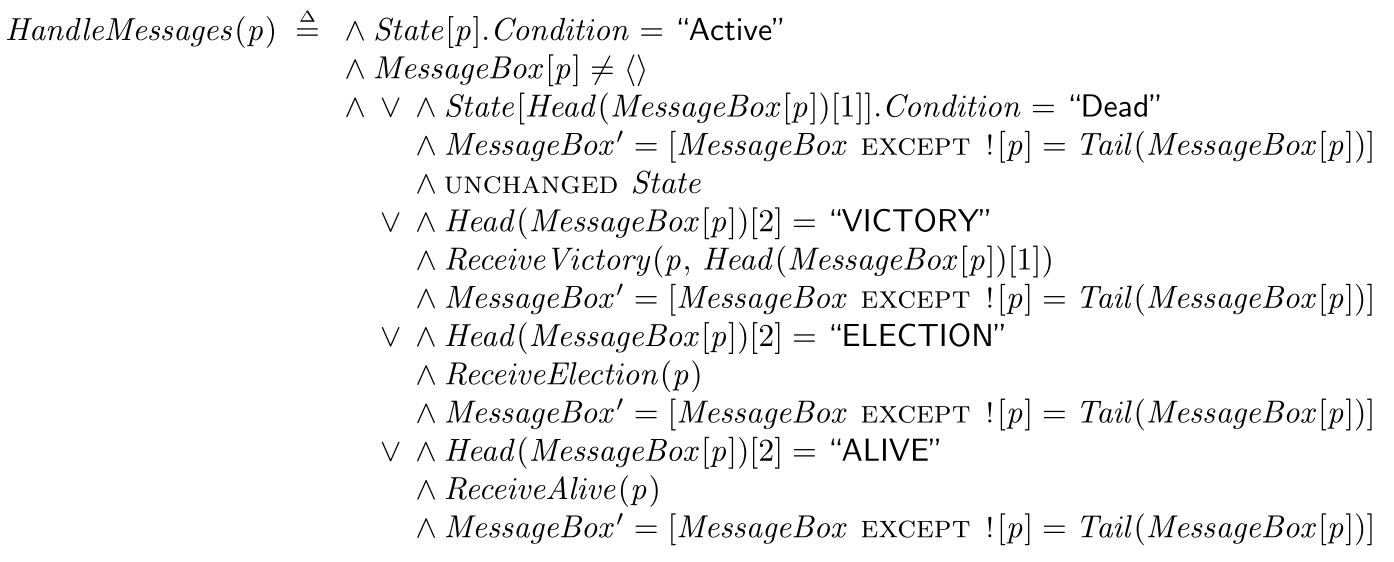
\includegraphics[scale=0.33]{handlemessages.png}} % scale to align
    }%
}

This function checks for new messages in a process' message box. It does this by looking at the first entry (the head) of the message box of process $p$. The first case is to clean up in case the process is dead. The only thing that is done, is to remove the message from the dead process. However, in the case where the process is not dead, the function looks at the contents of the message. It then calls the appropriate function depending the contents. After calling the function it removes the latest message by modifying the messagebox to be the tail.

\section{Checking the leader condition}
TODO: COnfidence 2/10: DÅrlig grammatik, dårlig formulering etc.\\
\noindent\fbox{%
    \parbox{\textwidth}{%
\makebox[\textwidth]{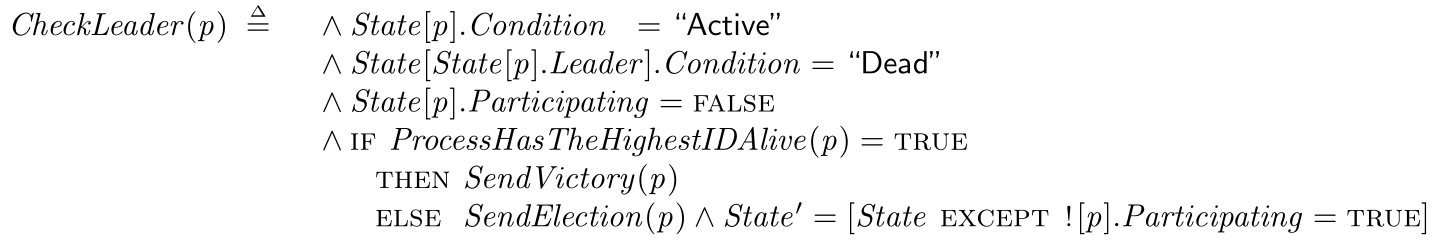
\includegraphics[scale=0.30]{checkleader.png}}
    }%
}

This function checks whether or not the current leader is dead. It only does this, if there is the process checking is not participating in an election (meaning that we assume there is no election). We then use the helper function defined up in the Sends, to see if the process has the highest ID. If this is the case, we just send a victory message, otherwise we send an election message out, and change the process to be participating in the election.
We can ``just'' say if the process has the highest ID, because we assume \textbf{TODO: hvad er det nu vi assumer siden vi bare kan sige det her? noget med at vi ved hvis processer er døde, vi ved bare ikke hvordan}
This is also the reason this function is used, rather than not getting a response and then assuming the leader process is dead.

\section{Next predicate and dying leader}
\begin{callout}
TODO: Confidence 2/10: For kort, dårligt beskrevet etc.
\end{callout}

\noindent\fbox{%
    \parbox{\textwidth}{%
\makebox[\textwidth]{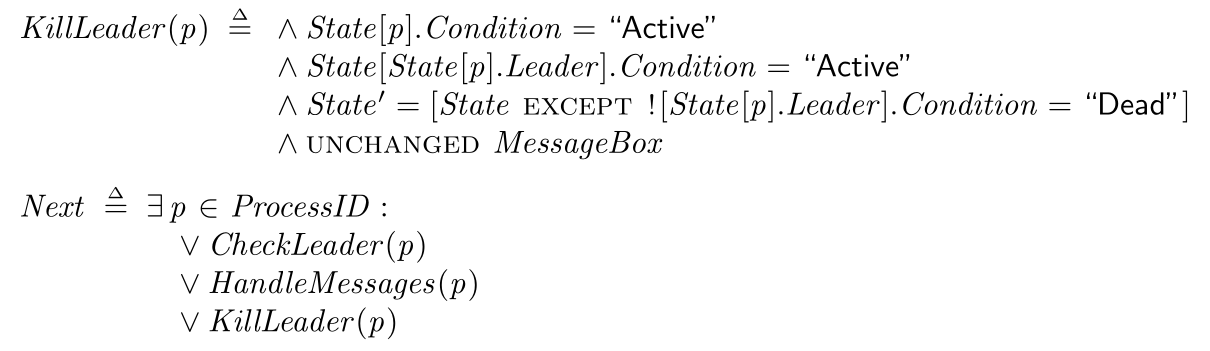
\includegraphics[scale=0.38]{killnext.png}}
    }%
}


The Next predicate is the predicate which chooses what should happen in the next state. Here we say that for some process $p$, we can either check if the leader is alive, handle any messages or kill the leader. Killing the leader is only a function to ensure the proper functioning of the spec.



\noindent\fbox{%
    \parbox{\textwidth}{%
\makebox[\textwidth]{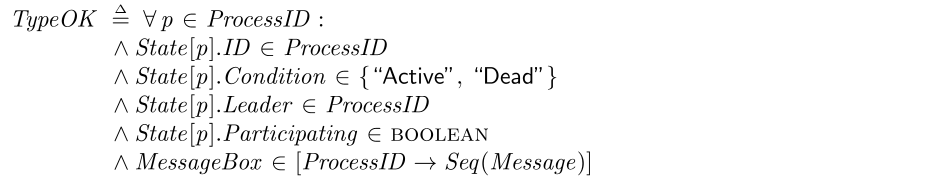
\includegraphics[scale=0.49]{typeok.png}}
\makebox[\textwidth]{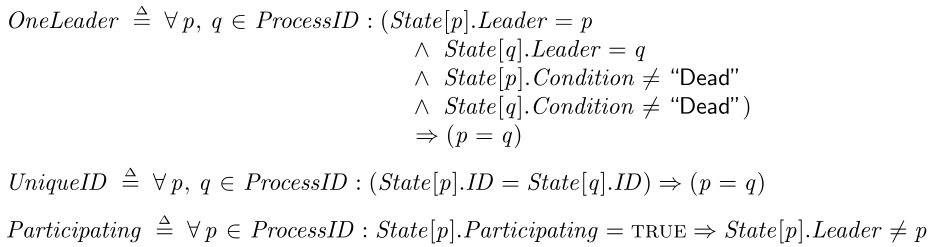
\includegraphics[scale=0.49]{t_invariants.png}}
    }%
}

\textbf{How the invariants are set up:}\\
The invariants are set up by depending on whether they are checking one process or two processes. If one process is checked, it checks for all processes p, while if they are checking two processes, they check for all processses p and q. Using this way, we make sure that each process gets treated correctly, and that we don't just select a random pair that might work at that moment.


Invariants will be checked to be true in every possible state.

Earlier in the report, we talked about TypeOK, as it is the invariant which makes sure that every variable holds legal values for this specification.
It does this by checking each process in ProcessID (I.e., each process in general) and making sure that they are a part of the correct set.(TODO: FOR PROCESSID THIS IS REDUNDANT). This means that the Condition proprety should either be Active or Dead, the leader should be a legal process id, participating should be a boolean and the messagebox should be a mapping from processid to a sequence of messages.

The OneLeader invariant makes sure that if there exists two leaders, then those two leaders must be the same process.
% TODO: This doesn't work, does it?
%
UniqueID makes sure that no process will have the same id.

Pariticpating makes sure that if a process is participating, it is not the leader itself.


\subsection{Properties}
..Explain what properties are...

There are two kinds of temporal properties: safety properties, and liveness properties. Safety properties make sure that the system doesn't do bad things, and liveness makes sure our system always does a good thing.\cite{https://learntla.com/core/temporal-logic.html}


\noindent\fbox{%
    \parbox{\textwidth}{%
\makebox[\textwidth]{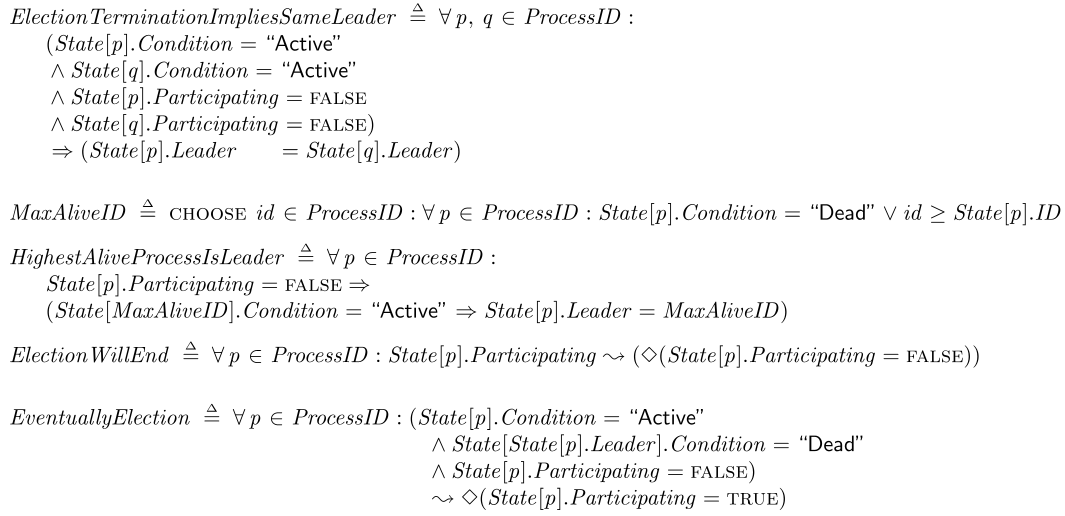
\includegraphics[scale=0.435]{properties.png}}
    }%
}

ElectionTerminationImpliesSameLeader is a safety property that ensures that when an election is done, everyone has the same leader.

HighestAliveProcessIsLeader is a safety property, tghat ensures that if a process is not participating in an election, then the highest alive process should be the leader.

ElectionWillEnd is a safety property that ensures that ensures that


\chapter{Ring Algorithm}

...Also called LCR

\section{Thought Process}

\lipsum[1]

\textbf{Similarities to Bully Algorithm}

The Ring Algorithm and the Bully Algorithm are both algorithms for leader election, and thus many of the core functions and models can be reused. These include invariants, properties, processes, messages and more.

\section{Setup}
\noindent\fbox{%
    \parbox{\textwidth}{%
\makebox[\textwidth]{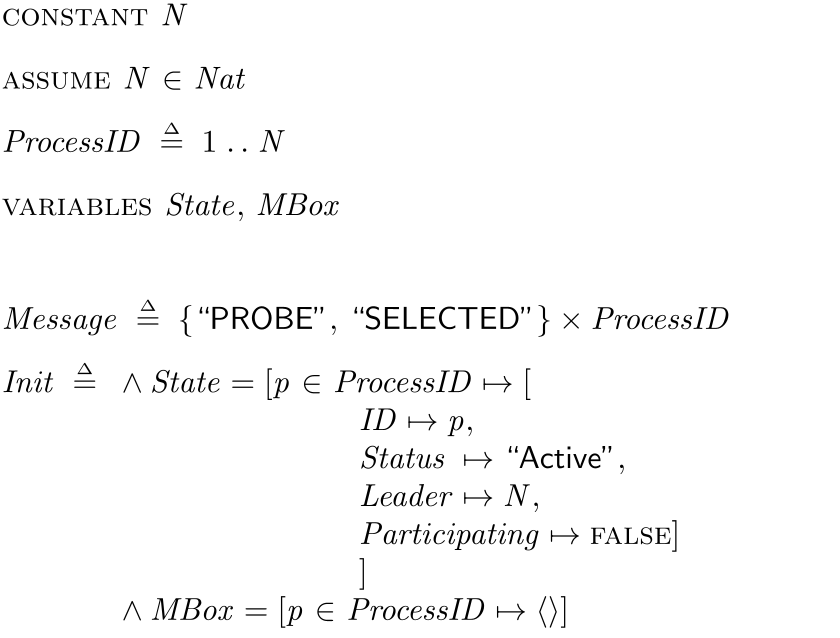
\includegraphics[scale=0.335]{ring_setup.png}}
    }%
}

This setup is a lot like the setup of the Bully Algorithm, except the Message function is different. This is solely a syntactic change. In the Ring algorithm each message holds an ``ID'', which is usually depicted as PROBE(ID) or SELECTED(ID). Thus, the change is made to reflect this, and also to avoid confusion with how the BullyAlgorithm handles it, where the process is the sender of the message, not the id. The sender isn't needed in the Ring Algorithm, as it is a ring structure and sends the message to the neighbour.

\section{Helper functions}
\noindent\fbox{%
    \parbox{\textwidth}{%
\makebox[\textwidth]{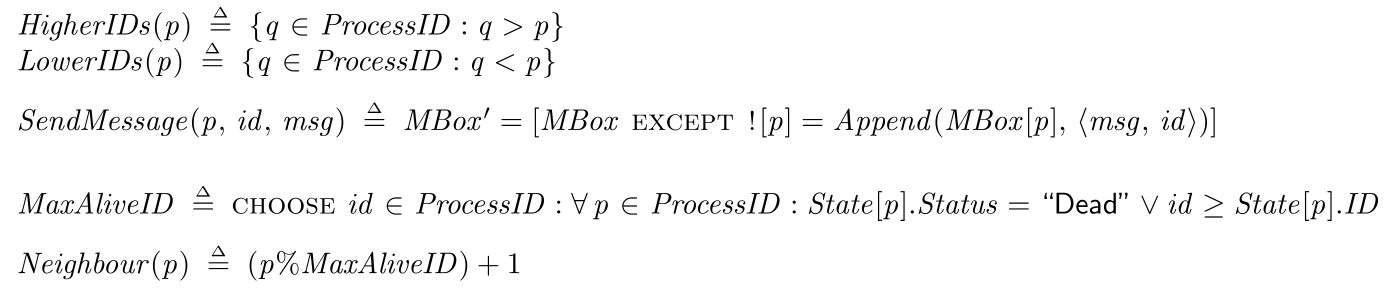
\includegraphics[scale=0.335]{ring_helpers.png}}
    }%
}


$$2+2 = 4$$
$2+2=4$
The helper functions are quite alike the helper functions in the bully algorithm as well, with the most noticable differences being the SendMessage and Neighbour functions.
The reason I decided for having a SendMessage function in the Ring Algorithm and not in Bully Algorithm, is that it aesthetically looks much prettier in the ring algorithm, and less cluttered, while it would only make it look more cluttered in the Bully Algorithm.
The neighbour function is a helper function for finding the right-side neighbour of the process. Since the algorithm assumes a ring structure, the right-hand neighbour is just the process id plus one. However, since a leader might die, this is divided with the MaxAliveID, to make sure that if the right hand neighbour is dead, it is sent to the lowest id instead. TODO: this should probably be changed, is in the real algorithm any process can die at any time.

\section{Event Handlers}
In the Ring algorithm there are two main events: receiving the Probe message and receiving the Selected message.

\noindent\fbox{%
    \parbox{\textwidth}{%
\makebox[\textwidth]{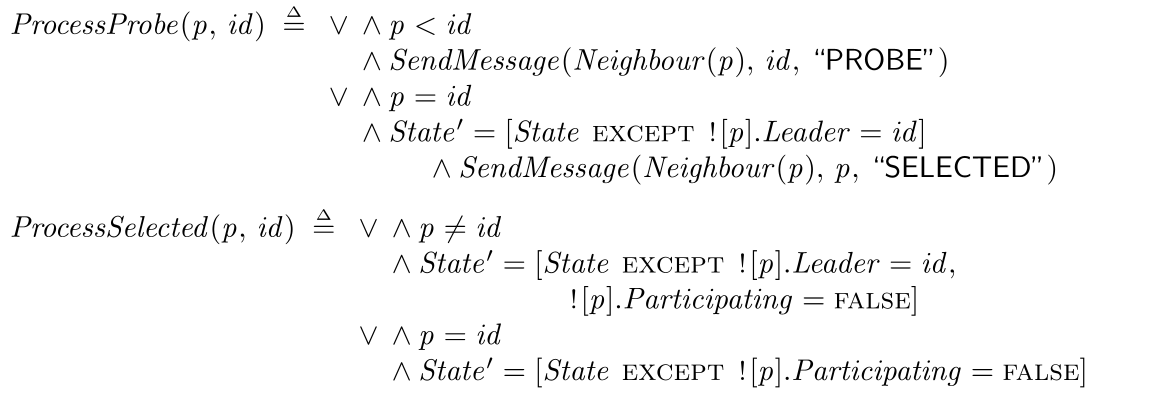
\includegraphics[scale=0.38]{ring_receive.png}}
    }%
}

\textbf{ProcessProbe}\\
According to the algorithm, in case a process receives a probe message, and the process id is lower than the id in the Probe message, the message is sent on the the next process. We do this using the SnedMessage and Neighbour helper functions. TODO: THIS IS WHERE THE PROBLEM HAPPENS PROBABLY. In the case of the ID being the same as the process ID, we assume that they are the new leader, and a SELECTED message with that process ID is sent, as well as their own leading being set to be themself. If the process ID is greater than the ID in the message, we do nothing, as is specified by the algorithm.

\textbf{ProcessSelected}\\
ProcessSelected simply checks if the process ID is equal to the ID of the Selected message. If so, the process is declared the election is done. Otherwise, the message is sent on, to keep declaring the new leader.


\section{HandleMessages}
\noindent\fbox{%
    \parbox{\textwidth}{%
\makebox[\textwidth]{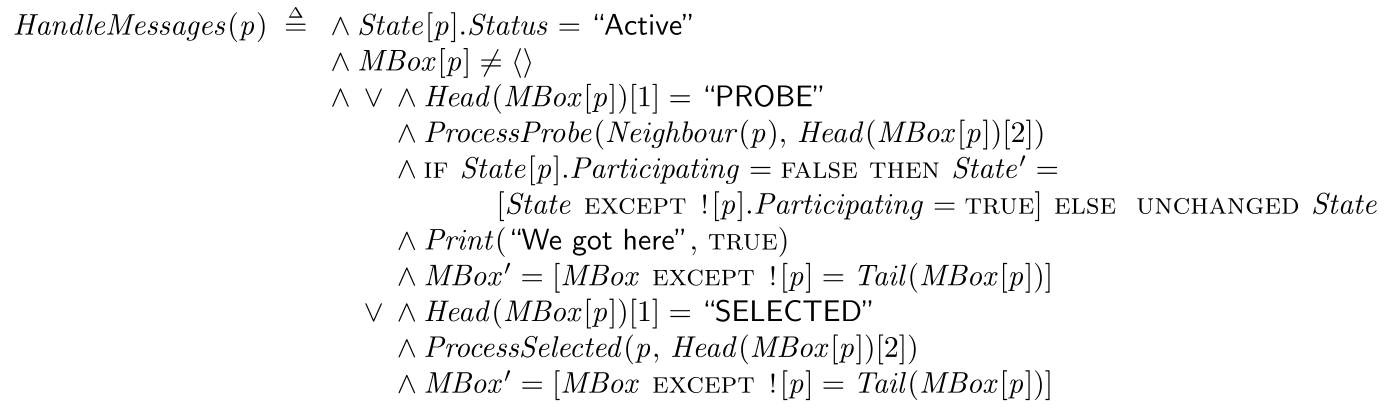
\includegraphics[scale=0.33]{ring_handle.png}}
    }%
}
TODO: Change image

HandleMessage is mostly identical to the HandleMessage functionp from the bully algorithm, except with changed messages, and in case of the message being a probe and the process' \textit{participating} field being false, we change it to true.

\section{Checking The Leader Condition}



\chapter{Evaluation}



\chapter{Conclusion}

...While the Bully Algorithm worked fine, the Ring Algorithm did not.

\bibliography{bibliography}

\appendix

\chapter{Bully Algorithm Implementation}



\chapter{Ring Algorithm Implementation}


\end{document}
